% Pregunta 1:

\textbf{(2pts.)} Considera la siguiente gram\'atica donde $E$ es el s\'imbolo
inicial:
\[
\begin{array}{rcl}
  E & \to & Aa\\
  A & \to & BC \mid BCf\\
  B & \to & b\\
  C & \to & c\\
\end{array}
\]
\begin{enumerate}
\item Construye los conjuntos can\'onicos de items \textbf{LR(0)}.
\item Con estos conjuntos construye el aut\'omtata finito mostrando las transiciones
  con la funci\'on GoTo.
\item Muestra la tabla de parsing que se genera usando el aut\'omata anterior. 
\end{enumerate}

\textbf{Solución.} Primero obtenemos la FNC
\[
\begin{array}{rcl}
  E  & \to & Aa\\
  A  & \to & BC \mid A'f\\
  A' & \to & BC\\
  B  & \to & b\\
  C  & \to & c\\
\end{array}
\]
Ahora encontremos los items asociados:
\[
I_0 = Closure(\{E' \rightarrow \text{\textbullet}E\}) = 
\begin{array}{rcl}
  E'  & \to & \text{\textbullet}E \\
  E  & \to & \text{\textbullet}Aa \\
  A  & \to & \text{\textbullet}BC \mid \text{\textbullet}A'f \\
  A' & \to & \text{\textbullet}BC\\
  B  & \to & \text{\textbullet}b \\
  C  & \to & \text{\textbullet}c \\
\end{array}
\]

Luego, para $I_1$
\[
I_1 = GoTo(\{I_0,E\}) = 
\begin{array}{rcl}
  E'  & \to & E\text{\textbullet}\\
  %E  & \to & A\text{\textbullet}a \\
  %A  & \to & \text{\textbullet}BC \mid \text{\textbullet}A'f \\
  %A' & \to & \text{\textbullet}BC\\
\end{array}
\]

así, tenemos que $I_2$
\[
I_2 = GoTo(\{I_0,A\}) = 
\begin{array}{rcl}
  %E  & \to & E\text{\textbullet}\\
  E  & \to & A\text{\textbullet}a \\
  %%A  & \to & B\text{\textbullet}C \mid A'\text{\textbullet}f \\
  %A' & \to & \text{\textbullet}BC\\
  %A' & \to & B\text{\textbullet}C\\
\end{array}
\]

observemos que $I_3$
\[
I_3 = GoTo(\{I_0,A'\}) = 
\begin{array}{rcl}
  %E  & \to & E\text{\textbullet}\\
  %E  & \to & A\text{\textbullet}a \\
  A  & \to &  A'\text{\textbullet}f \\ %B\text{\textbullet}C \mid
  %A' & \to & \text{\textbullet}BC\\
  %%A' & \to & B\text{\textbullet}C\\
\end{array}
\]


posteriormente, veamos que $I_4$
\[
I_4 = GoTo(\{I_0,B\}) = 
\begin{array}{rcl}
  %E  & \to & E\text{\textbullet}\\
  %E  & \to & A\text{\textbullet}a \\
  A  & \to & B\text{\textbullet}C\\
  A' & \to & B\text{\textbullet}C\\
  %%A' & \to & B\text{\textbullet}C\\
\end{array}
\]

y para $I_5$
\[
I_5 = GoTo(\{I_0,C\}) = 
\begin{array}{rcl}
  %E  & \to & E\text{\textbullet}\\
  %E  & \to & A\text{\textbullet}a \\
  A  & \to & BC\text{\textbullet}\\
  A' & \to & BC\text{\textbullet}\\
  %%A' & \to & B\text{\textbullet}C\\
\end{array}
\]

con $I_6$
\[
I_6 = GoTo(\{I_0,f\}) = 
\begin{array}{rcl}
  %E  & \to & E\text{\textbullet}\\
  %E  & \to & A\text{\textbullet}a \\
  A & \to & A'f\text{\textbullet}\\
\end{array}
\]

y para $I_7$
\[
I_7 = GoTo(\{I_0,a\}) = 
\begin{array}{rcl}
   E  & \to & Aa\text{\textbullet} \\
\end{array}
\]


con $I_8$
\[
I_8 = GoTo(\{I_0,b\}) = 
\begin{array}{rcl}
  B  & \to & b\text{\textbullet} \\
\end{array}
\]

Por último, tenemos que $I_9$
\[
I_9 = GoTo(\{I_0,c\}) = 
\begin{array}{rcl}
  C  & \to & \text{\textbullet}c \\
\end{array}
\]

A continuación se presenta el autómata generado por GoTo de R(0):
\begin{center}
        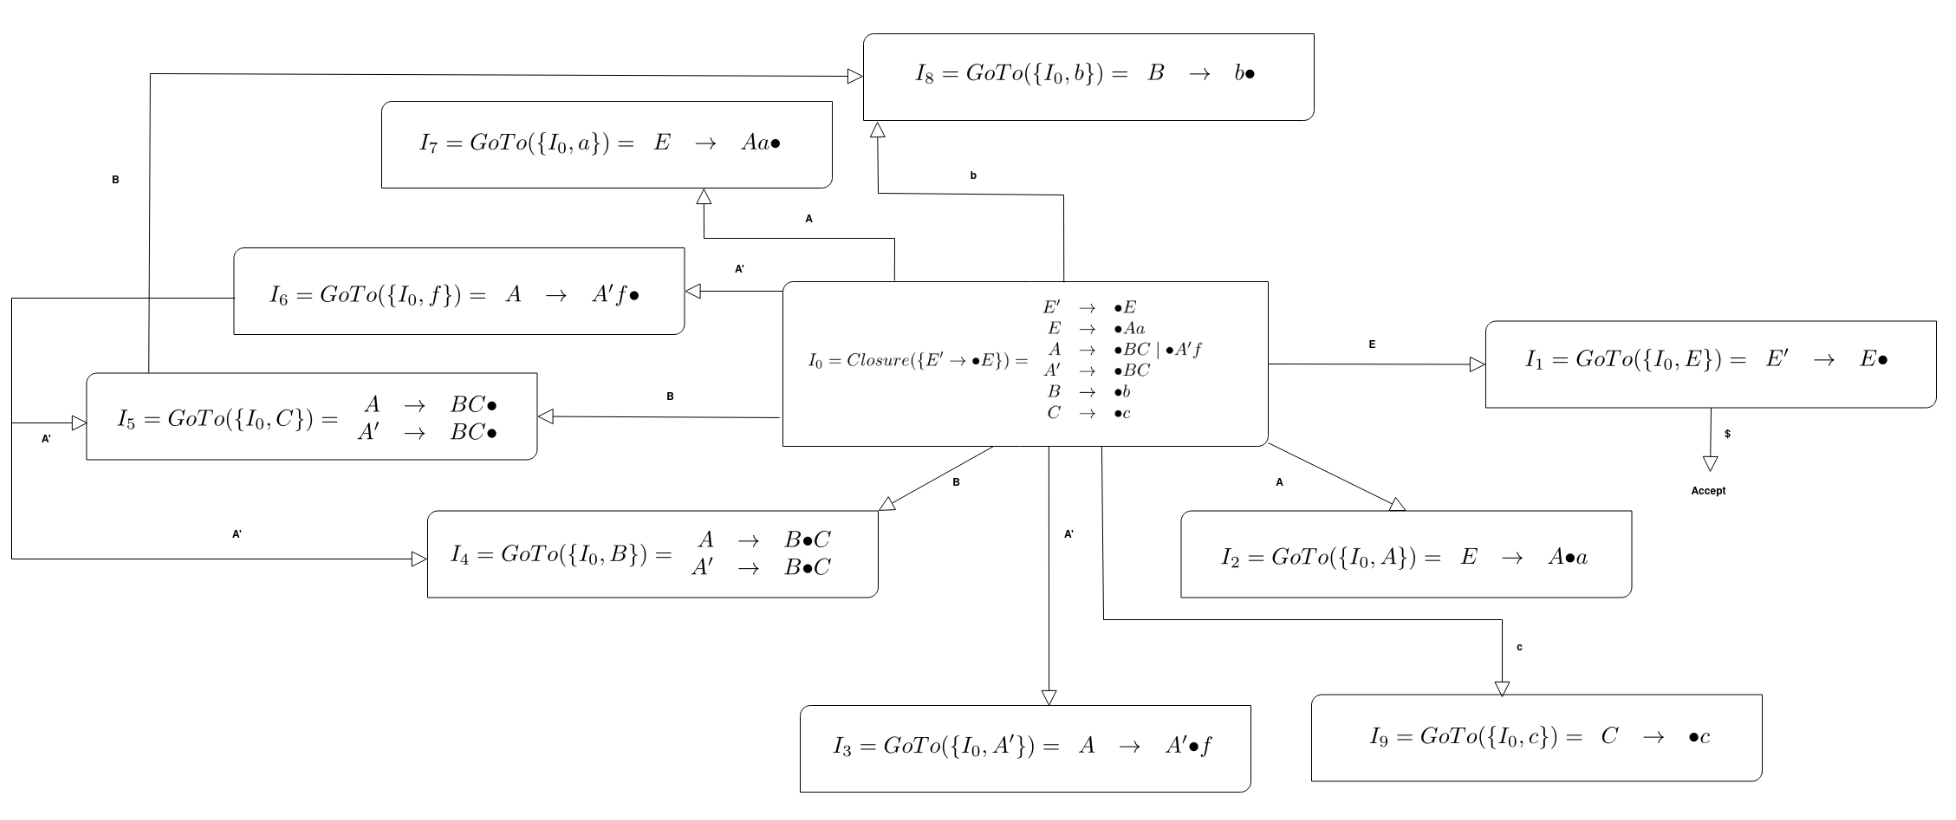
\includegraphics[scale=0.20]{./Im.png}\\[0.4cm]
\end{center}
 Para obtener la tabla de parsing supondremos que $0$ corresponde al estado de $I_0$
 y así para cada estado. A continuación se muestra la tabla de parsing.
\begin{center}
        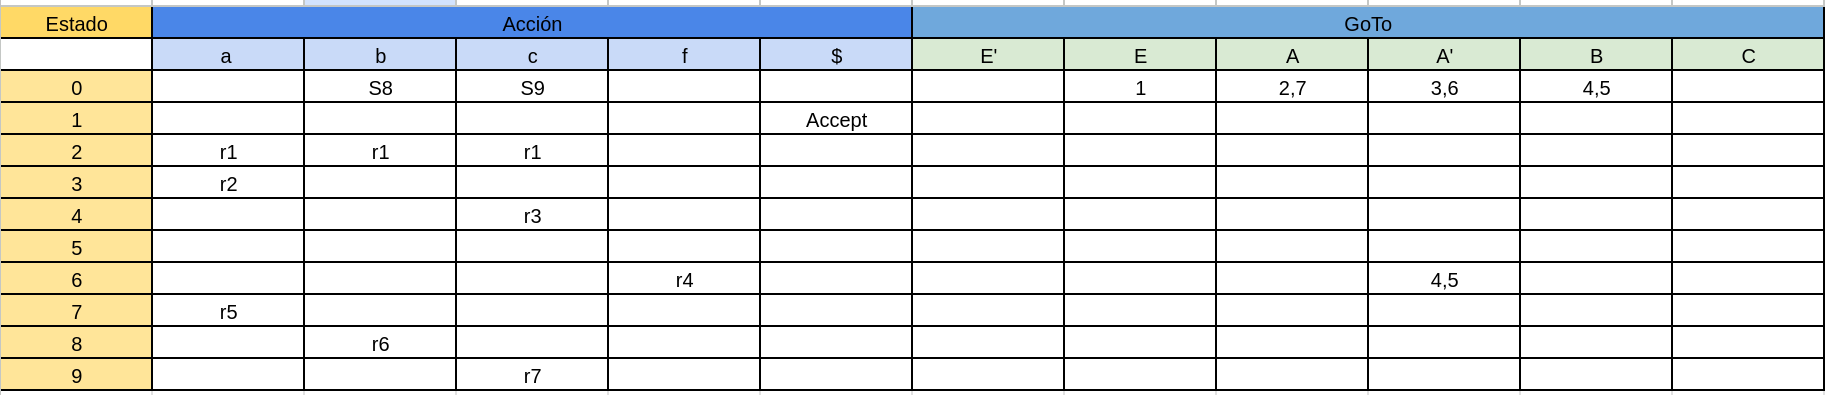
\includegraphics[scale=0.20]{./T1.png}\\[0.4cm]
\end{center}
